\chapter{Revisão de literatura}\label{chap:revisao}

Este capítulo apresenta a fundamentação teórica e tecnológica da proposta. A revisão foi organizada de forma narrativa, buscando relacionar conceitos de sensoriamento remoto, índices espectrais, imagens Sentinel-2, processamento geoespacial em nuvem e monitoramento agrícola.

\section{Estratégia de revisão}

A revisão de literatura foi organizada como revisão narrativa, com registro das fontes utilizadas e dos critérios de seleção. O objetivo não é executar uma revisão sistemática completa, mas reunir fundamentos técnicos e trabalhos relacionados suficientes para sustentar a proposta, delimitar o problema e justificar a metodologia.

As buscas priorizam fontes acadêmicas e documentação oficial. Para a fundamentação conceitual, são consideradas publicações sobre sensoriamento remoto, índices espectrais, agricultura de precisão e monitoramento de culturas. Para a parte tecnológica, são utilizadas documentações oficiais do Sentinel-2, Google Earth Engine e NASA POWER, além de materiais relacionados ao desenvolvimento em Python.

Quanto à atualidade, foram priorizadas referências publicadas nos últimos cinco anos, especialmente revisões e trabalhos relacionados ao uso de Sentinel-2, sensoriamento remoto agrícola e processamento geoespacial em nuvem. Referências mais antigas foram mantidas apenas quando representam bases conceituais consolidadas, como a formulação do NDVI, a formulação do NDWI e a descrição científica do Google Earth Engine. Essa combinação permite atender ao critério de atualidade sem substituir referências fundadoras por fontes secundárias menos adequadas.

Os critérios de inclusão são: relação direta com sensoriamento remoto agrícola, uso de índices espectrais, monitoramento de vegetação, processamento geoespacial em nuvem ou ferramentas utilizadas no sistema. Os critérios de exclusão são: fontes sem relação com agricultura ou vegetação, textos opinativos sem base técnica, materiais sem autoria ou procedência identificável e referências que não possam ser verificadas.

\section{Sensoriamento remoto aplicado à agricultura}

Sensoriamento remoto é a técnica de obter informações sobre objetos ou áreas da superfície terrestre sem contato físico direto. Em vez de coletar dados apenas por observação presencial, sensores instalados em satélites, aeronaves ou drones capturam a radiação refletida ou emitida pelos alvos. No contexto agrícola, essa abordagem permite analisar áreas extensas de forma recorrente, reduzindo a dependência de inspeções manuais para a observação inicial da lavoura.

O princípio central dessa aplicação é que diferentes alvos apresentam comportamentos distintos no espectro eletromagnético. A vegetação saudável tende a absorver fortemente a radiação na faixa do vermelho, devido à atividade fotossintética, e a refletir intensamente no infravermelho próximo, em função da estrutura interna das folhas. Já vegetações estressadas, solo exposto, água e áreas urbanizadas apresentam respostas espectrais diferentes. Essa diferença permite transformar medidas de reflectância em indicadores numéricos da condição da vegetação.

Em uma meta-revisão sobre aplicações agrícolas de sensoriamento remoto, \citet{WEISS2020} destacam que imagens orbitais têm sido empregadas em tarefas como estimativa de produtividade, monitoramento de desenvolvimento das culturas, avaliação de condições hídricas e acompanhamento de variáveis biofísicas. Essa literatura sustenta a escolha de uma abordagem baseada em imagens multiespectrais, pois o monitoramento agrícola depende da capacidade de observar variações espaciais e temporais que nem sempre são percebidas em inspeções pontuais de campo.

\begin{figure}[htb!]
    \centering
    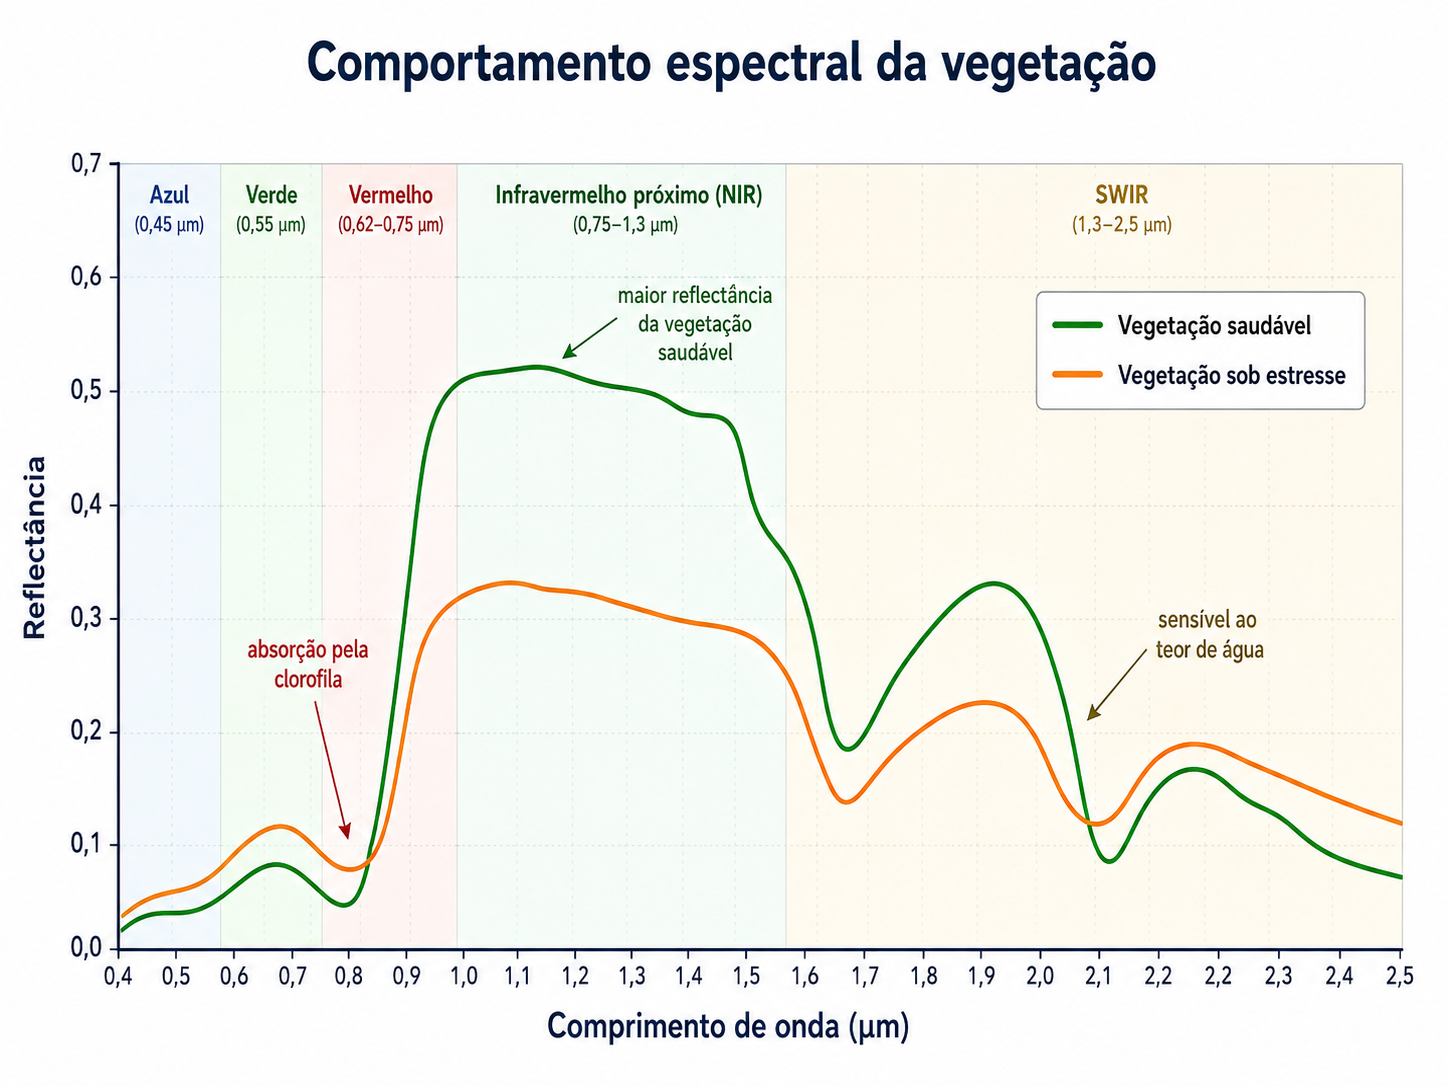
\includegraphics[width=0.88\textwidth]{fig/figura2.png}
    \caption{Comportamento espectral simplificado da vegetação saudável e da vegetação sob estresse.}
    \label{fig:comportamento-espectral}
    \vspace{0.2cm}
    \small Fonte: Adaptado de \citep{ROUSE1973,GAO1996}.
\end{figure}

No monitoramento agrícola, o sensoriamento remoto é útil para acompanhar desenvolvimento vegetativo, identificar variações espaciais dentro de talhões, observar possíveis falhas de plantio, detectar tendências de estresse e relacionar alterações da vegetação com eventos climáticos. Entretanto, seus resultados devem ser interpretados como indicadores indiretos. A imagem de satélite não identifica automaticamente a causa agronômica de um problema; ela aponta padrões que precisam ser analisados em conjunto com conhecimento de campo, histórico da cultura e dados complementares.

\section{Sentinel-2}

A missão Sentinel-2, pertencente ao programa Copernicus, é composta por satélites de imageamento multiespectral voltados ao monitoramento terrestre. A missão oferece alta frequência de revisita e bandas espectrais adequadas à análise de vegetação, solo, água e cobertura terrestre \citep{ESA_SENTINEL2}. O instrumento \textit{Multi-Spectral Instrument} registra bandas em resoluções espaciais de 10 m, 20 m e 60 m, abrangendo faixas do visível, infravermelho próximo e infravermelho de ondas curtas. A revisão apresentada por \citet{PHIRI2020} evidencia que os dados Sentinel-2 são amplamente utilizados em mapeamento e monitoramento de uso e cobertura da terra, o que reforça sua adequação para aplicações agrícolas baseadas em séries temporais e índices espectrais.

Para este trabalho, as bandas mais relevantes são a B4, correspondente ao vermelho, a B8, correspondente ao infravermelho próximo, e a B11, correspondente ao infravermelho de ondas curtas. A B4 e a B8 são utilizadas no cálculo do NDVI; a B8 e a B11 são utilizadas no cálculo do NDWI voltado à umidade da vegetação. A resolução espacial dessas bandas permite analisar talhões agrícolas, embora não permita a identificação de plantas individuais.

O uso de produtos de reflectância de superfície, como a coleção harmonizada Sentinel-2 MSI Level-2A disponível no Google Earth Engine, é adequado para análises temporais porque reduz efeitos atmosféricos em comparação com dados brutos. Ainda assim, é necessário aplicar filtros de data, área e cobertura de nuvens, pois nuvens e sombras podem distorcer o valor dos índices e gerar interpretações incorretas \citep{GOOGLE_S2_SR}.

\section{Índices espectrais}

Índices espectrais são combinações matemáticas entre bandas de uma imagem multiespectral. Seu objetivo é realçar determinadas características da superfície e reduzir a complexidade da análise, convertendo múltiplas bandas em um indicador numérico.

O NDVI é calculado pela razão normalizada entre o infravermelho próximo e o vermelho, conforme a \cref{eq:ndvi}.

\begin{equation}\label{eq:ndvi}
    NDVI = \frac{NIR - RED}{NIR + RED}
\end{equation}

O NDWI, na formulação de \citet{GAO1996} voltada à vegetação, utiliza o infravermelho próximo e o infravermelho de ondas curtas, conforme a \cref{eq:ndwi}.

\begin{equation}\label{eq:ndwi}
    NDWI = \frac{NIR - SWIR}{NIR + SWIR}
\end{equation}

Em imagens Sentinel-2, o NIR corresponde à banda B8 e o RED à banda B4. Valores próximos de zero indicam baixa presença de vegetação ou solo exposto; valores positivos mais altos indicam vegetação mais densa ou vigorosa; valores negativos costumam estar associados a água, nuvens ou superfícies não vegetadas. Em lavouras, o NDVI tende a variar ao longo do ciclo da cultura, crescendo durante o desenvolvimento vegetativo e reduzindo próximo à senescência ou colheita \citep{ROUSE1973}.

\begin{figure}[htb!]
    \centering
    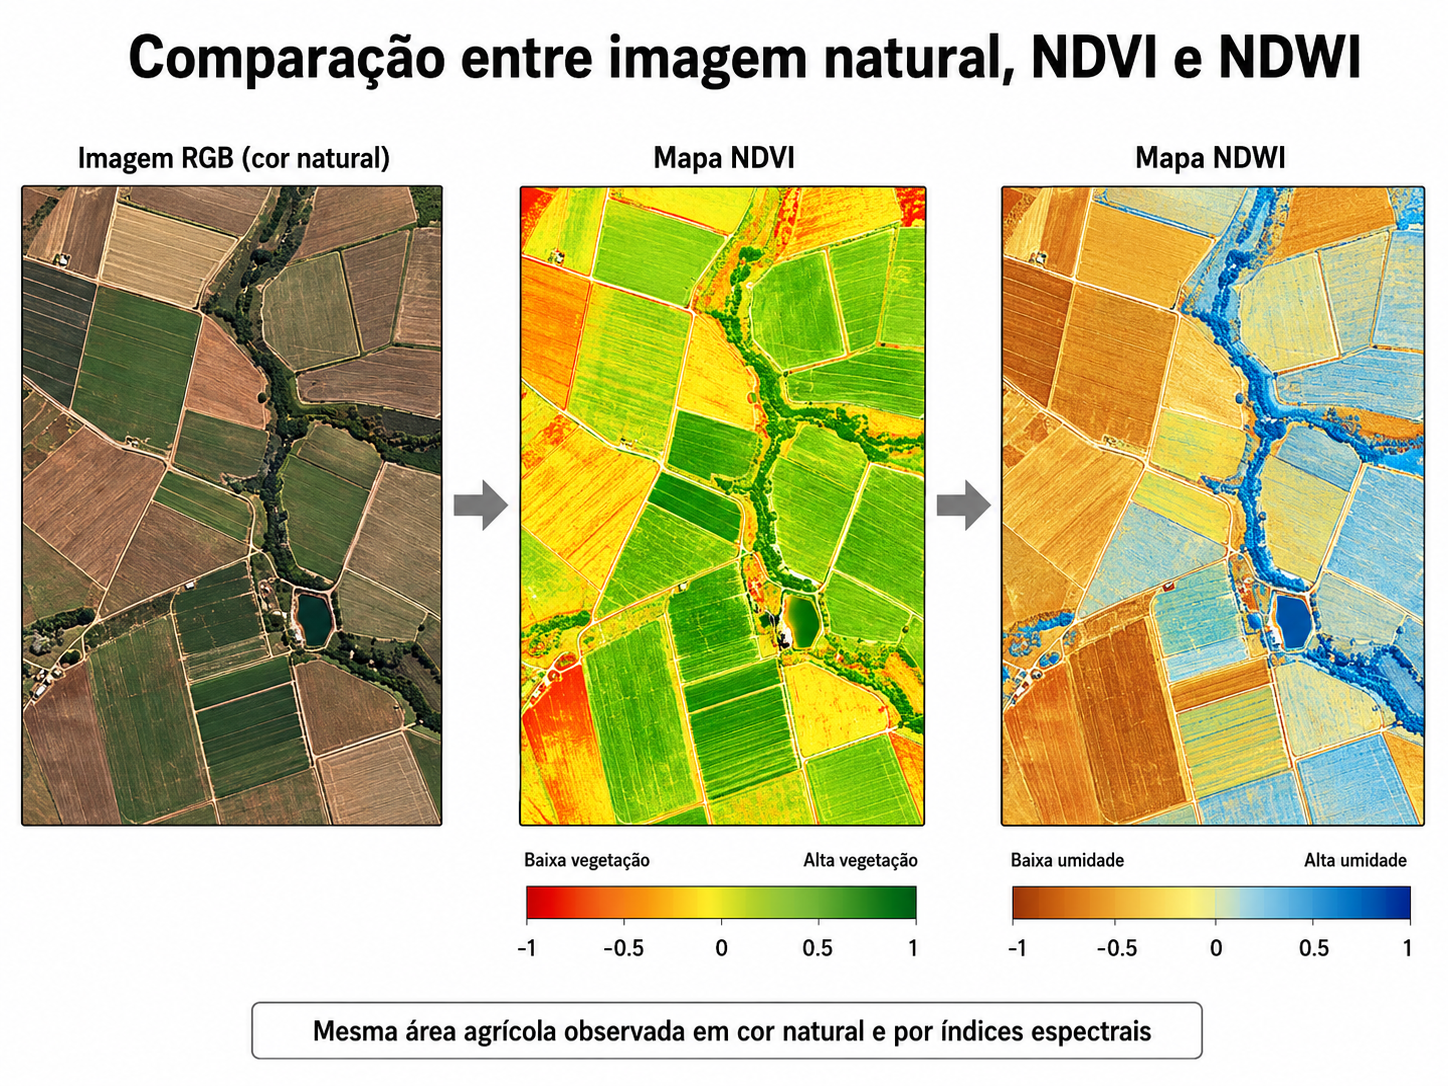
\includegraphics[width=0.94\textwidth]{fig/figura4.png}
    \caption{Comparação entre imagem em cor natural, NDVI e NDWI de uma área agrícola.}
    \label{fig:comparacao-rgb-ndvi-ndwi}
    \vspace{0.2cm}
    \small Fonte: Elaborado pelo autor a partir de dados Sentinel-2 (2026).
\end{figure}

No Sentinel-2, o NIR pode ser representado pela banda B8 e o SWIR pela banda B11. Esse índice é sensível ao conteúdo de água da vegetação, pois a reflectância no SWIR responde de maneira relevante à água presente nas folhas. Assim, valores baixos de NDWI podem sugerir menor teor de umidade ou possível estresse hídrico, especialmente quando interpretados junto com precipitação e temperatura.

Para este trabalho, NDVI e NDWI serão utilizados de forma complementar. O NDVI servirá como indicador principal de vigor da vegetação, enquanto o NDWI apoiará a análise de umidade. A interpretação conjunta reduz o risco de conclusões baseadas em um único indicador e ajuda a separar variações relacionadas ao crescimento normal da cultura de possíveis alterações associadas à disponibilidade hídrica.

\section{Google Earth Engine}

O Google Earth Engine é uma plataforma de processamento geoespacial em nuvem que disponibiliza catálogos de imagens de satélite e ferramentas para análise em larga escala. Seu uso é adequado para este trabalho porque evita a necessidade de baixar e armazenar localmente grandes volumes de imagens, transferindo operações como filtragem, composição, cálculo de índices e redução regional para servidores remotos \citep{GOOGLE_S2_SR}. A plataforma foi descrita por \citet{GORELICK2017} como uma infraestrutura para análise geoespacial em escala planetária, e revisões posteriores indicam sua adoção em diferentes aplicações de sensoriamento remoto com grandes volumes de dados \citep{AMANI2020}.

No sistema proposto, o Earth Engine será utilizado por meio da API Python. A aplicação consultará a coleção Sentinel-2, filtrará imagens por área, período e percentual de nuvens, calculará índices espectrais e retornará mapas ou estatísticas para a área de interesse. A função de diferença normalizada da plataforma permite implementar índices como NDVI e NDWI de forma direta, desde que as bandas corretas sejam informadas \citep{GOOGLE_EE_ND}.

Essa escolha tecnológica também contribui para a reprodutibilidade. Como os dados estão em uma coleção pública e as operações são definidas em código, a análise pode ser repetida para diferentes áreas e períodos, respeitando as limitações de disponibilidade de imagens e autenticação do serviço.

\section{Dados climáticos}

Dados climáticos são importantes para interpretar a dinâmica dos índices espectrais. Uma queda no NDVI, por exemplo, pode estar associada a senescência natural da cultura, colheita, falha de imagem, nuvens, seca, excesso de chuva, pragas ou outros fatores. A inclusão de variáveis como precipitação, temperatura e radiação solar não resolve automaticamente essa ambiguidade, mas fornece contexto adicional.

A NASA POWER disponibiliza dados meteorológicos e de radiação solar por meio de API, com parâmetros como precipitação diária, temperatura média e radiação solar de superfície \citep{NASA_POWER_DAILY}. No protótipo, a consulta será feita para o ponto central da área de interesse e para o mesmo intervalo temporal das imagens de satélite. Os dados serão apresentados em gráficos e comparados visualmente com as séries dos índices espectrais.

Essa integração permite que o usuário observe relações temporais, como queda de NDVI após período de baixa precipitação ou variações de vigor após mudanças climáticas. Ainda assim, a interpretação será apresentada como apoio à análise, não como diagnóstico causal definitivo.

\section{Sistemas de monitoramento agrícola e lacuna identificada}

Sistemas de monitoramento agrícola por sensoriamento remoto já são utilizados em diferentes níveis de complexidade. Soluções comerciais podem oferecer integração com mapas, sensores, maquinário, bancos de dados e alertas automáticos. Contudo, tais ferramentas podem apresentar custos, restrições de acesso ou complexidade incompatíveis com pequenos produtores, ambientes acadêmicos e protótipos de pesquisa.

O uso de visão computacional, inteligência artificial e sensoriamento remoto na agricultura de precisão tem sido discutido como uma linha relevante para culturas de grãos \citep{PATRICIO2018}. Além disso, estudos de revisão mostram que o sensoriamento remoto agrícola tem avançado tanto em métodos analíticos quanto na disponibilidade de dados orbitais gratuitos, especialmente com missões como Sentinel-2 e plataformas de processamento em nuvem \citep{WEISS2020,PHIRI2020,AMANI2020}. Entretanto, a lacuna explorada neste trabalho não é a criação de um método novo de sensoriamento remoto, mas a construção de um fluxo computacional integrado e reproduzível que demonstre, em escala de protótipo, como dados gratuitos podem ser organizados em uma aplicação prática.

Como síntese da revisão, observa-se que a literatura fornece três contribuições centrais para a metodologia proposta. Primeiro, os índices espectrais justificam tecnicamente o uso de bandas do vermelho, infravermelho próximo e infravermelho de ondas curtas para analisar vigor e umidade da vegetação. Segundo, o Sentinel-2 oferece dados multiespectrais gratuitos, com resolução e revisita compatíveis com o acompanhamento de áreas agrícolas. Terceiro, plataformas como o Google Earth Engine reduzem barreiras computacionais para consulta, filtragem e processamento das imagens. A partir dessas conclusões, o diferencial da proposta está na integração entre seleção de área, consulta de imagens Sentinel-2, cálculo de índices, visualização temporal, detecção simples de anomalias e comparação com clima em um sistema acessível. Assim, o trabalho se enquadra como pesquisa aplicada em Ciência da Computação, com desenvolvimento de artefato e validação por estudo de caso. Seu valor está em demonstrar a viabilidade técnica da solução e em documentar claramente os limites do protótipo para que ele possa ser evoluído em trabalhos futuros.
